\documentclass[11pt,aspectratio=169]{beamer}
\newcommand{\TalkShort}{Chapter 3: global transport}
% Visual reference: Matteo Di Sante, 13_06_26_slides_soaring_ctrw.tex.
% Steel-blue title bar, Palatino, Pisa seal, white pages and a pale title band.
\usepackage[T1]{fontenc}
\usepackage[utf8]{inputenc}
\usepackage[english]{babel}
\usepackage{mathpazo}
\usefonttheme{serif}
\usepackage{amsmath,amssymb,bm,booktabs,array,graphicx,tikz,microtype}
\usetikzlibrary{arrows.meta,calc,positioning}
\usepackage{siunitx}
\sisetup{group-separator={,},group-minimum-digits=4}
\usepackage{pgfpages}
\ifdefined\Speakernotes
  \setbeameroption{show notes on second screen=right}
\else
  \setbeameroption{hide notes}
\fi
\definecolor{pisablue}{RGB}{74,96,121}
\definecolor{pisablight}{RGB}{192,206,220}
\definecolor{accent}{RGB}{26,118,179}
\definecolor{para}{HTML}{3477A8}
\definecolor{hang}{HTML}{B5482A}
\definecolor{beginner}{HTML}{6A3D9A}
\definecolor{expert}{HTML}{C98A1E}
\definecolor{teal}{HTML}{2E7D8A}
\definecolor{wine}{HTML}{8E3B5C}
\definecolor{muted}{HTML}{666666}
\setbeamercolor{structure}{fg=pisablue}
\setbeamercolor{normal text}{fg=black,bg=white}
\setbeamercolor{frametitle}{fg=white,bg=pisablue}
\setbeamercolor{alerted text}{fg=accent}
\setbeamercolor{block title}{fg=white,bg=pisablue}
\setbeamercolor{block body}{fg=black,bg=pisablight!28}
\setbeamercolor{discussion}{fg=pisablue,bg=pisablight!30}
\setbeamercolor{button}{fg=white,bg=pisablue}
\setbeamerfont{button}{size=\normalsize}
\setbeamersize{text margin left=7mm,text margin right=7mm}
\setbeamertemplate{navigation symbols}{}
\setbeamertemplate{itemize item}{\textcolor{pisablue}{\small$\bullet$}}
\setbeamertemplate{itemize subitem}{\textcolor{pisablue}{\textendash}}
\setbeamertemplate{itemize/enumerate body begin}{\setlength{\itemsep}{0.55em}}
\setbeamertemplate{frametitle}{%
  \nointerlineskip
  \begin{beamercolorbox}[wd=\paperwidth,ht=9mm,dp=3mm,center]{frametitle}
    \large\insertframetitle\strut
  \end{beamercolorbox}
  \begin{tikzpicture}[remember picture,overlay]
    \node[anchor=north west,inner sep=0pt,xshift=2mm,yshift=-1.2mm]
      at(current page.north west){
\includegraphics[height=8mm]{assets/cherubino_white.png}};
    \node[anchor=north east,text=white,inner sep=0pt,xshift=-2.3mm,yshift=-4.2mm]
      at(current page.north east){\small\insertframenumber};
  \end{tikzpicture}
}
\setbeamertemplate{footline}{%
  \hspace{7mm}\textcolor{muted}{\fontsize{6.5}{8}\selectfont
    Matteo Di Sante\enspace|\enspace\TalkShort\enspace|\enspace13 September 2026}
  \hfill\textcolor{muted}{\fontsize{6.5}{8}\selectfont Supervisor discussion}\hspace{7mm}\vspace{2mm}
}
\newcommand{\kw}[1]{\textcolor{accent}{#1}}
\newcommand{\source}[1]{\par\vspace{1mm}{\fontsize{7}{8.3}\selectfont\color{muted}#1\par}}
\newcommand{\question}[1]{\par\vfill
  \begin{beamercolorbox}[wd=\linewidth,sep=5pt]{discussion}
    \small #1
  \end{beamercolorbox}}
\newcommand{\fig}[2][54mm]{\includegraphics[width=\linewidth,height=#1,keepaspectratio]{assets/#2}\par}
\newcommand{\speaker}[1]{\note{#1}}
\setbeamertemplate{note page}{%
  \vspace{4mm}\noindent%
  \begin{minipage}{\linewidth}
    {\small\color{pisablue}\TalkShort\quad|\quad Slide \insertframenumber}\par\medskip
    {\normalsize\bfseries\insertframetitle}\par\medskip
    {\small\insertnote}
  \end{minipage}
}
\newcommand{\refitem}[3]{\href{#1}{#2}\hfill {\color{muted}#3}\par\medskip}
\newcommand{\titleframe}[4]{%
\begin{frame}[plain]
\begin{tikzpicture}[remember picture,overlay]
 \fill[pisablue](current page.south west)rectangle(current page.north east);
 \fill[pisablight](current page.south west)rectangle([yshift=20mm]current page.south east);
 \node[anchor=north,yshift=-4mm]at(current page.north){
\includegraphics[height=13mm]{assets/cherubino_white.png}};
 \node[text=white,align=center]at([yshift=19mm]current page.center)
   {{\scshape\large University of Pisa}\\[2mm]{\small Department of Physics ``Enrico Fermi''}};
 \node[text=white,align=center,text width=.92\paperwidth]at([yshift=-3mm]current page.center)
   {{\LARGE\bfseries #1}\\[3mm]{\large #2}};
 \node[text=pisablue,align=center]at([yshift=10mm]current page.south)
   {{\normalsize Matteo Di Sante}\quad$\bullet$\quad{\normalsize 13 September 2026}\\[2mm]
    {\small #3}};
\end{tikzpicture}
\note{#4}
\end{frame}}
\newcommand{\backupstart}{%
\appendix
\begin{frame}[plain,noframenumbering]
\begin{tikzpicture}[remember picture,overlay]
 \fill[pisablue](current page.south west)rectangle(current page.north east);
 \node[text=white,align=center]at(current page.center)
  {{\LARGE\bfseries Discussion material}\\[4mm]{\large Extra figures, derivations and references}};
\end{tikzpicture}
\end{frame}}
\hypersetup{colorlinks=true,urlcolor=accent,linkcolor=accent,pdfauthor={Matteo Di Sante}}
% A notes sheet contains a second rendering of the slide. Disable its duplicate
% destinations; the normal slide PDF retains all hyperlinks and the viewer button.
\ifdefined\Speakernotes\hypersetup{draft}\fi

% Generated by scripts/reporting/ch3_global_transport/generate_revision_diagnostics.py -- do not edit.
\newcommand{\StatRevParaFlights}{155085}
\newcommand{\StatRevParaFixedFlights}{14360}
\newcommand{\StatRevParaLastFlights}{68207}
\newcommand{\StatRevParaLastWindows}{84997}
\newcommand{\StatRevParaLastOrderTwoFlights}{14360}
\newcommand{\StatRevParaAlphaOne}{1.703}
\newcommand{\StatRevParaAlphaTwo}{2.003}
\newcommand{\StatRevParaResidualOne}{0.050}
\newcommand{\StatRevParaResidualTwo}{0.071}
\newcommand{\StatRevParaFixedAlphaOne}{1.790}
\newcommand{\StatRevParaFixedAlphaTwo}{2.059}
\newcommand{\StatRevParaMomentZetaTwo}{1.737}
\newcommand{\StatRevParaMomentNuMin}{0.843}
\newcommand{\StatRevParaMomentNuMax}{0.883}
\newcommand{\StatRevParaMardiaMin}{-2.05}
\newcommand{\StatRevParaMardiaMedian}{0.67}
\newcommand{\StatRevParaMardiaMax}{5.91}
\newcommand{\StatRevParaOpenFlights}{67003}
\newcommand{\StatRevParaOpenAlphaOne}{1.770}
\newcommand{\StatRevParaOpenAlphaTwo}{1.937}
\newcommand{\StatRevParaOpenClosure}{0.365}
\newcommand{\StatRevParaClosedFlights}{87807}
\newcommand{\StatRevParaClosedAlphaOne}{1.623}
\newcommand{\StatRevParaClosedAlphaTwo}{2.036}
\newcommand{\StatRevParaClosedClosure}{0.027}
\newcommand{\StatRevParaEastLower}{0.811}
\newcommand{\StatRevParaEastMedian}{0.840}
\newcommand{\StatRevParaEastUpper}{0.844}
\newcommand{\StatRevParaEastNinetieth}{0.852}
\newcommand{\StatRevParaNorthLower}{0.837}
\newcommand{\StatRevParaNorthMedian}{0.858}
\newcommand{\StatRevParaNorthUpper}{0.863}
\newcommand{\StatRevParaNorthNinetieth}{0.878}
\newcommand{\StatRevParaRadialLower}{0.835}
\newcommand{\StatRevParaRadialMedian}{0.840}
\newcommand{\StatRevParaRadialUpper}{0.859}
\newcommand{\StatRevParaRadialNinetieth}{0.879}
\newcommand{\StatRevParaNarrowRadialLower}{0.975}
\newcommand{\StatRevParaNarrowRadialMedian}{0.895}
\newcommand{\StatRevParaNarrowRadialUpper}{0.862}
\newcommand{\StatRevParaNarrowRadialNinetieth}{0.872}
\newcommand{\StatRevParaQuantileFixedFlights}{14360}
\newcommand{\StatRevParaQuantileFixedOrigins}{21739115}
\newcommand{\StatRevParaQuantileControlFitMinS}{10}
\newcommand{\StatRevParaQuantileControlFitMaxS}{10000}
\newcommand{\StatRevParaQuantileChangingLower}{0.835}
\newcommand{\StatRevParaQuantileChangingMedian}{0.840}
\newcommand{\StatRevParaQuantileChangingUpper}{0.859}
\newcommand{\StatRevParaQuantileChangingNinetieth}{0.879}
\newcommand{\StatRevParaQuantileControlledLower}{0.976}
\newcommand{\StatRevParaQuantileControlledMedian}{0.899}
\newcommand{\StatRevParaQuantileControlledUpper}{0.890}
\newcommand{\StatRevParaQuantileControlledNinetieth}{0.898}
\newcommand{\StatRevParaDurationOneHFlights}{146786}
\newcommand{\StatRevParaDurationOneHRatio}{1.00}
\newcommand{\StatRevParaDurationTwoHFlights}{101980}
\newcommand{\StatRevParaDurationTwoHRatio}{1.09}
\newcommand{\StatRevParaDurationFourHFlights}{34594}
\newcommand{\StatRevParaDurationFourHRatio}{1.40}
\newcommand{\StatRevParaVacfTenAtSixHundred}{0.128}
\newcommand{\StatRevParaVacfSixtyAtSixHundred}{0.180}
\newcommand{\StatRevParaVacfThreeHundredAtSixHundred}{0.252}
\newcommand{\StatRevParaDurationReferenceLagS}{1070}
\newcommand{\StatRevHangFlights}{6060}
\newcommand{\StatRevHangFixedFlights}{563}
\newcommand{\StatRevHangLastFlights}{3313}
\newcommand{\StatRevHangLastWindows}{3920}
\newcommand{\StatRevHangLastOrderTwoFlights}{563}
\newcommand{\StatRevHangAlphaOne}{1.649}
\newcommand{\StatRevHangAlphaTwo}{1.985}
\newcommand{\StatRevHangResidualOne}{0.065}
\newcommand{\StatRevHangResidualTwo}{0.075}
\newcommand{\StatRevHangFixedAlphaOne}{1.744}
\newcommand{\StatRevHangFixedAlphaTwo}{2.025}
\newcommand{\StatRevHangMomentZetaTwo}{1.682}
\newcommand{\StatRevHangMomentNuMin}{0.832}
\newcommand{\StatRevHangMomentNuMax}{0.854}
\newcommand{\StatRevHangMardiaMin}{-1.64}
\newcommand{\StatRevHangMardiaMedian}{1.52}
\newcommand{\StatRevHangMardiaMax}{8.38}
\newcommand{\StatRevHangOpenFlights}{2183}
\newcommand{\StatRevHangOpenAlphaOne}{1.688}
\newcommand{\StatRevHangOpenAlphaTwo}{1.892}
\newcommand{\StatRevHangOpenClosure}{0.177}
\newcommand{\StatRevHangClosedFlights}{3877}
\newcommand{\StatRevHangClosedAlphaOne}{1.628}
\newcommand{\StatRevHangClosedAlphaTwo}{2.007}
\newcommand{\StatRevHangClosedClosure}{0.026}
\newcommand{\StatRevHangEastLower}{0.803}
\newcommand{\StatRevHangEastMedian}{0.806}
\newcommand{\StatRevHangEastUpper}{0.800}
\newcommand{\StatRevHangEastNinetieth}{0.817}
\newcommand{\StatRevHangNorthLower}{0.869}
\newcommand{\StatRevHangNorthMedian}{0.879}
\newcommand{\StatRevHangNorthUpper}{0.839}
\newcommand{\StatRevHangNorthNinetieth}{0.839}
\newcommand{\StatRevHangRadialLower}{0.860}
\newcommand{\StatRevHangRadialMedian}{0.829}
\newcommand{\StatRevHangRadialUpper}{0.821}
\newcommand{\StatRevHangRadialNinetieth}{0.845}
\newcommand{\StatRevHangNarrowRadialLower}{1.001}
\newcommand{\StatRevHangNarrowRadialMedian}{0.909}
\newcommand{\StatRevHangNarrowRadialUpper}{0.833}
\newcommand{\StatRevHangNarrowRadialNinetieth}{0.839}
\newcommand{\StatRevHangQuantileFixedFlights}{563}
\newcommand{\StatRevHangQuantileFixedOrigins}{791712}
\newcommand{\StatRevHangQuantileControlFitMinS}{10}
\newcommand{\StatRevHangQuantileControlFitMaxS}{10000}
\newcommand{\StatRevHangQuantileChangingLower}{0.860}
\newcommand{\StatRevHangQuantileChangingMedian}{0.829}
\newcommand{\StatRevHangQuantileChangingUpper}{0.821}
\newcommand{\StatRevHangQuantileChangingNinetieth}{0.845}
\newcommand{\StatRevHangQuantileControlledLower}{1.000}
\newcommand{\StatRevHangQuantileControlledMedian}{0.895}
\newcommand{\StatRevHangQuantileControlledUpper}{0.863}
\newcommand{\StatRevHangQuantileControlledNinetieth}{0.868}
\newcommand{\StatRevHangDurationOneHFlights}{5835}
\newcommand{\StatRevHangDurationOneHRatio}{1.01}
\newcommand{\StatRevHangDurationTwoHFlights}{4581}
\newcommand{\StatRevHangDurationTwoHRatio}{1.12}
\newcommand{\StatRevHangDurationFourHFlights}{1719}
\newcommand{\StatRevHangDurationFourHRatio}{1.50}
\newcommand{\StatRevHangVacfTenAtSixHundred}{0.124}
\newcommand{\StatRevHangVacfSixtyAtSixHundred}{0.173}
\newcommand{\StatRevHangVacfThreeHundredAtSixHundred}{0.249}
\newcommand{\StatRevHangDurationReferenceLagS}{1070}
\newcommand{\StatRevParaPcaReferenceLagS}{1000}
\newcommand{\StatRevParaPcaAlpsFlights}{90737}
\newcommand{\StatRevParaPcaAlpsRatio}{2.13}
\newcommand{\StatRevParaPcaAlpsAngle}{65.7}
\newcommand{\StatRevParaPcaPyreneesFlights}{12242}
\newcommand{\StatRevParaPcaPyreneesRatio}{2.19}
\newcommand{\StatRevParaPcaPyreneesAngle}{169.5}
\newcommand{\StatRevParaPcaChannelCoastFlights}{4890}
\newcommand{\StatRevParaPcaChannelCoastRatio}{1.92}
\newcommand{\StatRevParaPcaChannelCoastAngle}{29.7}
\newcommand{\StatRevHangPcaReferenceLagS}{1000}
\newcommand{\StatRevHangPcaAlpsFlights}{4535}
\newcommand{\StatRevHangPcaAlpsRatio}{1.55}
\newcommand{\StatRevHangPcaAlpsAngle}{85.0}
\newcommand{\StatRevHangPcaPyreneesFlights}{181}
\newcommand{\StatRevHangPcaPyreneesRatio}{1.68}
\newcommand{\StatRevHangPcaPyreneesAngle}{162.1}
\newcommand{\StatRevHangPcaChannelCoastFlights}{26}
\newcommand{\StatRevHangPcaChannelCoastRatio}{2.11}
\newcommand{\StatRevHangPcaChannelCoastAngle}{40.4}

% Generated by scripts/reporting/ch3_global_transport/generate_duration_equipment.py -- do not edit.
\newcommand{\StatDurationParaFlights}{155085}
\newcommand{\StatDurationHangFlights}{6060}
\newcommand{\StatDurationABFullExponent}{1.728}
\newcommand{\StatDurationCDCCCFullExponent}{1.788}
\newcommand{\StatDurationFullFitMinS}{10}
\newcommand{\StatDurationFullFitMaxS}{10000}
\newcommand{\StatDurationFitMinS}{10}
\newcommand{\StatDurationFitMaxS}{1695}
\newcommand{\StatDurationMinFlights}{30}
\newcommand{\StatDurationUnknownFlights}{6510}

% Generated by scripts/reporting/ch3_global_transport/generate_kinematic_isotropy_figure.py -- do not edit.
\newcommand{\StatKinFitMinS}{10}
\newcommand{\StatKinFitMaxS}{10000}
\newcommand{\StatKinMinFlights}{30}
\newcommand{\StatKinMinClusters}{10}
\newcommand{\StatKinParaFlights}{156406}
\newcommand{\StatKinParaPositionMedian}{0.82}
\newcommand{\StatKinParaPositionMin}{0.72}
\newcommand{\StatKinParaPositionMax}{0.87}
\newcommand{\StatKinParaVelocityMedian}{0.89}
\newcommand{\StatKinParaVelocityMin}{0.84}
\newcommand{\StatKinParaVelocityMax}{0.95}
\newcommand{\StatKinParaAccelerationMedian}{0.97}
\newcommand{\StatKinParaAccelerationMin}{0.95}
\newcommand{\StatKinParaAccelerationMax}{0.99}
\newcommand{\StatKinTerrainAlpsFlights}{91932}
\newcommand{\StatKinTerrainAlpsPositionMedian}{0.67}
\newcommand{\StatKinTerrainAlpsPositionMin}{0.60}
\newcommand{\StatKinTerrainAlpsPositionMax}{0.83}
\newcommand{\StatKinTerrainAlpsVelocityMedian}{0.81}
\newcommand{\StatKinTerrainAlpsVelocityMin}{0.68}
\newcommand{\StatKinTerrainAlpsVelocityMax}{0.92}
\newcommand{\StatKinTerrainAlpsAccelerationMedian}{0.97}
\newcommand{\StatKinTerrainAlpsAccelerationMin}{0.94}
\newcommand{\StatKinTerrainAlpsAccelerationMax}{1.00}
\newcommand{\StatKinTerrainAlpsEquipmentABFlights}{36605}
\newcommand{\StatKinTerrainAlpsEquipmentABPositionMedian}{0.61}
\newcommand{\StatKinTerrainAlpsEquipmentABPositionMin}{0.53}
\newcommand{\StatKinTerrainAlpsEquipmentABPositionMax}{0.75}
\newcommand{\StatKinTerrainAlpsEquipmentABVelocityMedian}{0.79}
\newcommand{\StatKinTerrainAlpsEquipmentABVelocityMin}{0.63}
\newcommand{\StatKinTerrainAlpsEquipmentABVelocityMax}{0.86}
\newcommand{\StatKinTerrainAlpsEquipmentABAccelerationMedian}{0.96}
\newcommand{\StatKinTerrainAlpsEquipmentABAccelerationMin}{0.91}
\newcommand{\StatKinTerrainAlpsEquipmentABAccelerationMax}{1.02}
\newcommand{\StatKinTerrainAlpsEquipmentCDCCCFlights}{51358}
\newcommand{\StatKinTerrainAlpsEquipmentCDCCCPositionMedian}{0.70}
\newcommand{\StatKinTerrainAlpsEquipmentCDCCCPositionMin}{0.62}
\newcommand{\StatKinTerrainAlpsEquipmentCDCCCPositionMax}{0.89}
\newcommand{\StatKinTerrainAlpsEquipmentCDCCCVelocityMedian}{0.83}
\newcommand{\StatKinTerrainAlpsEquipmentCDCCCVelocityMin}{0.71}
\newcommand{\StatKinTerrainAlpsEquipmentCDCCCVelocityMax}{0.97}
\newcommand{\StatKinTerrainAlpsEquipmentCDCCCAccelerationMedian}{0.97}
\newcommand{\StatKinTerrainAlpsEquipmentCDCCCAccelerationMin}{0.93}
\newcommand{\StatKinTerrainAlpsEquipmentCDCCCAccelerationMax}{1.01}
\newcommand{\StatKinTerrainPyreneesFlights}{12330}
\newcommand{\StatKinTerrainPyreneesPositionMedian}{1.67}
\newcommand{\StatKinTerrainPyreneesPositionMin}{1.21}
\newcommand{\StatKinTerrainPyreneesPositionMax}{5.05}
\newcommand{\StatKinTerrainPyreneesVelocityMedian}{1.19}
\newcommand{\StatKinTerrainPyreneesVelocityMin}{1.00}
\newcommand{\StatKinTerrainPyreneesVelocityMax}{1.39}
\newcommand{\StatKinTerrainPyreneesAccelerationMedian}{0.99}
\newcommand{\StatKinTerrainPyreneesAccelerationMin}{0.91}
\newcommand{\StatKinTerrainPyreneesAccelerationMax}{1.07}
\newcommand{\StatKinTerrainPyreneesEquipmentABFlights}{3971}
\newcommand{\StatKinTerrainPyreneesEquipmentABPositionMedian}{1.78}
\newcommand{\StatKinTerrainPyreneesEquipmentABPositionMin}{1.12}
\newcommand{\StatKinTerrainPyreneesEquipmentABPositionMax}{5.05}
\newcommand{\StatKinTerrainPyreneesEquipmentABVelocityMedian}{1.13}
\newcommand{\StatKinTerrainPyreneesEquipmentABVelocityMin}{0.98}
\newcommand{\StatKinTerrainPyreneesEquipmentABVelocityMax}{1.50}
\newcommand{\StatKinTerrainPyreneesEquipmentABAccelerationMedian}{0.98}
\newcommand{\StatKinTerrainPyreneesEquipmentABAccelerationMin}{0.89}
\newcommand{\StatKinTerrainPyreneesEquipmentABAccelerationMax}{1.08}
\newcommand{\StatKinTerrainPyreneesEquipmentCDCCCFlights}{7964}
\newcommand{\StatKinTerrainPyreneesEquipmentCDCCCPositionMedian}{1.60}
\newcommand{\StatKinTerrainPyreneesEquipmentCDCCCPositionMin}{1.22}
\newcommand{\StatKinTerrainPyreneesEquipmentCDCCCPositionMax}{5.11}
\newcommand{\StatKinTerrainPyreneesEquipmentCDCCCVelocityMedian}{1.20}
\newcommand{\StatKinTerrainPyreneesEquipmentCDCCCVelocityMin}{1.01}
\newcommand{\StatKinTerrainPyreneesEquipmentCDCCCVelocityMax}{1.35}
\newcommand{\StatKinTerrainPyreneesEquipmentCDCCCAccelerationMedian}{0.99}
\newcommand{\StatKinTerrainPyreneesEquipmentCDCCCAccelerationMin}{0.92}
\newcommand{\StatKinTerrainPyreneesEquipmentCDCCCAccelerationMax}{1.07}
\newcommand{\StatKinTerrainChannelCoastFlights}{4963}
\newcommand{\StatKinTerrainChannelCoastPositionMedian}{0.96}
\newcommand{\StatKinTerrainChannelCoastPositionMin}{0.89}
\newcommand{\StatKinTerrainChannelCoastPositionMax}{1.09}
\newcommand{\StatKinTerrainChannelCoastVelocityMedian}{0.97}
\newcommand{\StatKinTerrainChannelCoastVelocityMin}{0.90}
\newcommand{\StatKinTerrainChannelCoastVelocityMax}{1.11}
\newcommand{\StatKinTerrainChannelCoastAccelerationMedian}{0.97}
\newcommand{\StatKinTerrainChannelCoastAccelerationMin}{0.88}
\newcommand{\StatKinTerrainChannelCoastAccelerationMax}{1.07}
\newcommand{\StatKinTerrainChannelCoastEquipmentABFlights}{879}
\newcommand{\StatKinTerrainChannelCoastEquipmentABPositionMedian}{1.12}
\newcommand{\StatKinTerrainChannelCoastEquipmentABPositionMin}{0.76}
\newcommand{\StatKinTerrainChannelCoastEquipmentABPositionMax}{1.75}
\newcommand{\StatKinTerrainChannelCoastEquipmentABVelocityMedian}{0.97}
\newcommand{\StatKinTerrainChannelCoastEquipmentABVelocityMin}{0.74}
\newcommand{\StatKinTerrainChannelCoastEquipmentABVelocityMax}{1.38}
\newcommand{\StatKinTerrainChannelCoastEquipmentABAccelerationMedian}{0.96}
\newcommand{\StatKinTerrainChannelCoastEquipmentABAccelerationMin}{0.72}
\newcommand{\StatKinTerrainChannelCoastEquipmentABAccelerationMax}{1.20}
\newcommand{\StatKinTerrainChannelCoastEquipmentCDCCCFlights}{3789}
\newcommand{\StatKinTerrainChannelCoastEquipmentCDCCCPositionMedian}{0.98}
\newcommand{\StatKinTerrainChannelCoastEquipmentCDCCCPositionMin}{0.92}
\newcommand{\StatKinTerrainChannelCoastEquipmentCDCCCPositionMax}{1.09}
\newcommand{\StatKinTerrainChannelCoastEquipmentCDCCCVelocityMedian}{0.98}
\newcommand{\StatKinTerrainChannelCoastEquipmentCDCCCVelocityMin}{0.90}
\newcommand{\StatKinTerrainChannelCoastEquipmentCDCCCVelocityMax}{1.10}
\newcommand{\StatKinTerrainChannelCoastEquipmentCDCCCAccelerationMedian}{0.97}
\newcommand{\StatKinTerrainChannelCoastEquipmentCDCCCAccelerationMin}{0.87}
\newcommand{\StatKinTerrainChannelCoastEquipmentCDCCCAccelerationMax}{1.10}
\newcommand{\StatKinEquipmentABFlights}{54574}
\newcommand{\StatKinEquipmentABPositionMedian}{0.74}
\newcommand{\StatKinEquipmentABPositionMin}{0.65}
\newcommand{\StatKinEquipmentABPositionMax}{0.80}
\newcommand{\StatKinEquipmentABVelocityMedian}{0.85}
\newcommand{\StatKinEquipmentABVelocityMin}{0.78}
\newcommand{\StatKinEquipmentABVelocityMax}{0.91}
\newcommand{\StatKinEquipmentABAccelerationMedian}{0.97}
\newcommand{\StatKinEquipmentABAccelerationMin}{0.93}
\newcommand{\StatKinEquipmentABAccelerationMax}{1.00}
\newcommand{\StatKinEquipmentCDCCCFlights}{95157}
\newcommand{\StatKinEquipmentCDCCCPositionMedian}{0.86}
\newcommand{\StatKinEquipmentCDCCCPositionMin}{0.74}
\newcommand{\StatKinEquipmentCDCCCPositionMax}{0.91}
\newcommand{\StatKinEquipmentCDCCCVelocityMedian}{0.91}
\newcommand{\StatKinEquipmentCDCCCVelocityMin}{0.86}
\newcommand{\StatKinEquipmentCDCCCVelocityMax}{0.97}
\newcommand{\StatKinEquipmentCDCCCAccelerationMedian}{0.98}
\newcommand{\StatKinEquipmentCDCCCAccelerationMin}{0.94}
\newcommand{\StatKinEquipmentCDCCCAccelerationMax}{1.00}
\newcommand{\StatKinHangFlights}{6094}
\newcommand{\StatKinHangPositionMedian}{1.03}
\newcommand{\StatKinHangPositionMin}{0.54}
\newcommand{\StatKinHangPositionMax}{1.45}
\newcommand{\StatKinHangVelocityMedian}{1.05}
\newcommand{\StatKinHangVelocityMin}{0.76}
\newcommand{\StatKinHangVelocityMax}{1.19}
\newcommand{\StatKinHangAccelerationMedian}{1.01}
\newcommand{\StatKinHangAccelerationMin}{0.86}
\newcommand{\StatKinHangAccelerationMax}{1.16}

% Generated by scripts/reporting/ch3_global_transport/generate_msd_figure.py -- do not edit.
\newcommand{\StatMsdParaAlpha}{1.920}
\newcommand{\StatMsdParaAlphaErr}{0.001}
\newcommand{\StatMsdParaAlphaErrOls}{0.016}
\newcommand{\StatMsdParaHurst}{0.960}
\newcommand{\StatMsdParaFitMinS}{121}
\newcommand{\StatMsdParaFitMaxS}{13021}
\newcommand{\StatMsdParaFlights}{156406}
\newcommand{\StatMsdParaSegments}{194048}
\newcommand{\StatMsdTaParaAlpha}{1.779}
\newcommand{\StatMsdTaParaAlphaErr}{0.000}
\newcommand{\StatMsdTaParaAlphaErrOls}{0.004}
\newcommand{\StatMsdTaParaHurst}{0.889}
\newcommand{\StatMsdTaParaFitMinS}{10}
\newcommand{\StatMsdTaParaFitMaxS}{10000}
\newcommand{\StatMsdParaAlphaGap}{0.141}
\newcommand{\StatMsdParaAlphaEast}{1.917}
\newcommand{\StatMsdParaAlphaEastErr}{0.002}
\newcommand{\StatMsdParaAlphaEastErrOls}{0.015}
\newcommand{\StatMsdParaHurstEast}{0.958}
\newcommand{\StatMsdParaHurstEastErr}{0.001}
\newcommand{\StatMsdParaAlphaNorth}{1.922}
\newcommand{\StatMsdParaAlphaNorthErr}{0.002}
\newcommand{\StatMsdParaAlphaNorthErrOls}{0.017}
\newcommand{\StatMsdParaHurstNorth}{0.961}
\newcommand{\StatMsdParaHurstNorthErr}{0.001}
\newcommand{\StatMsdTaParaAlphaEast}{1.754}
\newcommand{\StatMsdTaParaAlphaEastErr}{0.001}
\newcommand{\StatMsdTaParaAlphaEastErrOls}{0.004}
\newcommand{\StatMsdTaParaHurstEast}{0.877}
\newcommand{\StatMsdTaParaHurstEastErr}{0.000}
\newcommand{\StatMsdTaParaAlphaNorth}{1.797}
\newcommand{\StatMsdTaParaAlphaNorthErr}{0.001}
\newcommand{\StatMsdTaParaAlphaNorthErrOls}{0.004}
\newcommand{\StatMsdTaParaHurstNorth}{0.898}
\newcommand{\StatMsdTaParaHurstNorthErr}{0.000}
\newcommand{\StatMsdParaAlphaGapEast}{0.162}
\newcommand{\StatMsdParaAlphaGapNorth}{0.126}
\newcommand{\StatMsdParaCohortSpread}{0.008}
\newcommand{\StatMsdParaCohortSpreadNaive}{0.055}
\newcommand{\StatMsdParaCohortCount}{3}
\newcommand{\StatMsdParaCohortMaxH}{4}
\newcommand{\StatMsdParaCohortAlphaOneH}{1.865}
\newcommand{\StatMsdParaCohortAlphaTwoH}{1.896}
\newcommand{\StatMsdParaCohortAlphaFourH}{1.928}
\newcommand{\StatMsdTaParaCohortSpread}{0.028}
\newcommand{\StatMsdTaParaCohortSpreadNaive}{0.022}
\newcommand{\StatMsdTaParaCohortCount}{3}
\newcommand{\StatMsdTaParaCohortMaxH}{4}
\newcommand{\StatMsdTaParaCohortAlphaOneH}{1.791}
\newcommand{\StatMsdTaParaCohortAlphaTwoH}{1.784}
\newcommand{\StatMsdTaParaCohortAlphaFourH}{1.801}
\newcommand{\StatMsdHangAlpha}{1.901}
\newcommand{\StatMsdHangAlphaErr}{0.008}
\newcommand{\StatMsdHangAlphaErrOls}{0.030}
\newcommand{\StatMsdHangHurst}{0.951}
\newcommand{\StatMsdHangFitMinS}{121}
\newcommand{\StatMsdHangFitMaxS}{14680}
\newcommand{\StatMsdHangFlights}{6094}
\newcommand{\StatMsdHangSegments}{7662}
\newcommand{\StatMsdTaHangAlpha}{1.737}
\newcommand{\StatMsdTaHangAlphaErr}{0.003}
\newcommand{\StatMsdTaHangAlphaErrOls}{0.005}
\newcommand{\StatMsdTaHangHurst}{0.868}
\newcommand{\StatMsdTaHangFitMinS}{10}
\newcommand{\StatMsdTaHangFitMaxS}{10000}
\newcommand{\StatMsdHangAlphaGap}{0.165}
\newcommand{\StatMsdHangAlphaEast}{1.809}
\newcommand{\StatMsdHangAlphaEastErr}{0.012}
\newcommand{\StatMsdHangAlphaEastErrOls}{0.026}
\newcommand{\StatMsdHangHurstEast}{0.904}
\newcommand{\StatMsdHangHurstEastErr}{0.006}
\newcommand{\StatMsdHangAlphaNorth}{1.987}
\newcommand{\StatMsdHangAlphaNorthErr}{0.011}
\newcommand{\StatMsdHangAlphaNorthErrOls}{0.037}
\newcommand{\StatMsdHangHurstNorth}{0.994}
\newcommand{\StatMsdHangHurstNorthErr}{0.006}
\newcommand{\StatMsdTaHangAlphaEast}{1.708}
\newcommand{\StatMsdTaHangAlphaEastErr}{0.004}
\newcommand{\StatMsdTaHangAlphaEastErrOls}{0.007}
\newcommand{\StatMsdTaHangHurstEast}{0.854}
\newcommand{\StatMsdTaHangHurstEastErr}{0.002}
\newcommand{\StatMsdTaHangAlphaNorth}{1.758}
\newcommand{\StatMsdTaHangAlphaNorthErr}{0.003}
\newcommand{\StatMsdTaHangAlphaNorthErrOls}{0.004}
\newcommand{\StatMsdTaHangHurstNorth}{0.879}
\newcommand{\StatMsdTaHangHurstNorthErr}{0.002}
\newcommand{\StatMsdHangAlphaGapEast}{0.100}
\newcommand{\StatMsdHangAlphaGapNorth}{0.229}
\newcommand{\StatMsdHangCohortSpread}{0.027}
\newcommand{\StatMsdHangCohortSpreadNaive}{0.082}
\newcommand{\StatMsdHangCohortCount}{3}
\newcommand{\StatMsdHangCohortMaxH}{4}
\newcommand{\StatMsdHangCohortAlphaOneH}{1.820}
\newcommand{\StatMsdHangCohortAlphaTwoH}{1.896}
\newcommand{\StatMsdHangCohortAlphaFourH}{1.878}
\newcommand{\StatMsdTaHangCohortSpread}{0.029}
\newcommand{\StatMsdTaHangCohortSpreadNaive}{0.023}
\newcommand{\StatMsdTaHangCohortCount}{3}
\newcommand{\StatMsdTaHangCohortMaxH}{4}
\newcommand{\StatMsdTaHangCohortAlphaOneH}{1.758}
\newcommand{\StatMsdTaHangCohortAlphaTwoH}{1.747}
\newcommand{\StatMsdTaHangCohortAlphaFourH}{1.759}

\hypersetup{pdftitle={Global transport: measurements, controls and open model questions}}

\begin{document}
% MAIN TALK: 18 slides, 20 minutes including the final discussion prompt.
\titleframe{Global transport in soaring flights}
  {Measurements, controls and open model questions}
  {Chapter 3\enspace$\bullet$\enspace20-minute supervisor meeting}
\timing{0:20}{The purpose is to agree which empirical constraints can support model comparison now, and which controls are needed before rejecting a stochastic process. The earlier CTRW slides supply the visual style only; their proposed model and universality claims are not results of this analysis.}

\begin{frame}{What motion should a stochastic model reproduce?}
\begin{columns}[T,onlytextwidth]
\column{.56\textwidth}
\[
 \mathbf X_f(t,\tau)=\mathbf r_f(t+\tau)-\mathbf r_f(t),\qquad R_f=|\mathbf X_f|.
\]
\[
 M_2^{\rm flight}(\tau)=\frac{1}{N_f(\tau)}
       \sum_f\underbrace{\frac1{n_f(\tau)}\sum_k R_{fk}^2}_{\text{mean within flight }f}.
\]
\small Windows stay within a retained segment. The main comparison covers
\kw{$10\le\tau\le10^4$ s}.
\column{.40\textwidth}
\small
\textbf{Two levels of evidence}\par\medskip
Archive: \num{\StatMsdParaFlights} paragliders and \num{\StatMsdHangFlights} hang gliders.\par\medskip
Detailed diagnostics: \StatRevParaFlights\ and \StatRevHangFlights\ selected flights, one longest segment per flight, on a 10-s grid.
\end{columns}
\question{Displacement growth, distribution shape, directional preference and memory must be confronted together.}
\source{Archive baseline: equal segment weights. Subset $V_1,V_2$: equal flight weights. Baseline quantiles and moments: pooled windows.}
\timing{1:00}{Define horizontal position in a local east--north frame. The archive's original time-average curve uses equal segments, while the detailed subset and duration report use equal flights. The baseline high-order moments and quantiles pool windows. These distinctions explain why slopes from different figures are not interchangeable. The subset is reproducible but not a simple random sample of every flight. Flights recorded more slowly than 10 seconds are omitted. Launch-synchronised averages mix locations, years and seasons, so their difference from time averages is not an ergodicity test.}
\end{frame}

\begin{frame}{The MSD grows faster than linearly on the measured interval}
\begin{columns}[c,onlytextwidth]
\column{.67\textwidth}
\centering\fig[53mm]{scaling-top.pdf}
\column{.30\textwidth}
\small
\begin{tabular}{@{}lcc@{}}\toprule
 & $b_1$ & $b_2$\\\midrule
\textcolor{para}{Para} & \StatRevParaAlphaOne & \StatRevParaAlphaTwo\\
\textcolor{hang}{Hang} & \StatRevHangAlphaOne & \StatRevHangAlphaTwo\\\bottomrule
\end{tabular}
\medskip\par
$V_1=\langle R^2\rangle$; $V_2$ uses second differences.\par\medskip
The local slope bends. One fitted number does not establish a power law.
\end{columns}
\source{Subset; 10--10,000 s. Solid: $V_1$; dashed: $V_2$; dotted: $V_1$, fixed long cohort. Right: half the local slope. Descriptive fits; no calibrated confidence intervals.}
\timing{1:10}{Start from the observable, not a Hurst label. The first-difference exponents are 1.702 and 1.662 in this subset. The full archive's equal-segment time averages have descriptive slopes 1.779 and 1.742 under a different estimator. The plotted local slopes change with lag. Native cadence and smoothing matter near the lower end; changing flight coverage matters near the upper end. Introduce V2 only as the constant-velocity control explained next.}
\end{frame}

\begin{frame}{Second differences cancel constant velocity; an intrinsic $H$ remains open}
\[
 A_2\mathbf r=\mathbf r(t+2\tau)-2\mathbf r(t+\tau)+\mathbf r(t),
 \qquad V_2=\langle|A_2\mathbf r|^2\rangle.
\]
\begin{columns}[T,onlytextwidth]
\column{.48\textwidth}
\textbf{Exact cancellation}\par
\[
 \mathbf r(t)=\mathbf r_0+\mathbf v_dt+\mathbf Y(t)
 \quad\Rightarrow\quad A_2\mathbf r=A_2\mathbf Y.
\]
\small The constant velocity may combine wind, route choice and net progress. A turn or spatially varying wind survives.
\column{.48\textwidth}
\textbf{Conditional interpretation}\par
\small If the centred residual has stationary increments and variance $K\tau^{2H}$,
\[
 V_2=K(4-2^{2H})\tau^{2H},\quad 0<H<1.
\]
At $H=1$ the prefactor vanishes. Our $b_2\simeq2$ cannot be read as a validated $H\simeq1$.
\end{columns}
\question{Which residual and which scale interval could satisfy the assumptions needed to estimate $H$?}
\source{At $\tau=10^4$ s, $V_2$ retains only 107 para / 56 hang flights; it needs $2\tau$ of continuous support.}
\timing{1:20}{Explain the cancellation algebraically. Adjacent increments I1 and I2 obey Var(I1+I2)=K(2tau) to the power 2H. Expanding Var(I2-I1) gives the prefactor. The derivation requires finite variance and stationary increments with the stated power over the relevant lags, including 2tau. A smooth curved trajectory instead gives V2 proportional to tau to the fourth at small lag. We have therefore gained a diagnostic invariant, but have not isolated the motion in still air or obtained its Hurst exponent.}
\end{frame}

\begin{frame}{Open and closed tasks change the growth of displacements}
\begin{columns}[c,onlytextwidth]
\column{.42\textwidth}
\centering
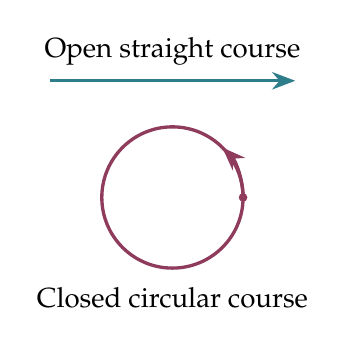
\begin{tikzpicture}[scale=.78,>=Stealth]
 \draw[teal,line width=1.2pt,->](-2,1.6)--(2,1.6);
 \node[above]at(0,1.7){Open straight course};
 \draw[wine,line width=1.2pt](0,-.3)circle(1.15);
 \fill[wine](1.15,-.3)circle(2pt);
 \draw[wine,->,line width=1.2pt](1.15,-.3)arc(0:45:1.15);
 \node[below]at(0,-1.6){Closed circular course};
\end{tikzpicture}
\column{.54\textwidth}
\small\textbf{Measured subset}\par\medskip
\begin{tabular}{@{}llrrr@{}}\toprule
 & Task & $N$ & $b_1$ & $b_2$\\\midrule
Para & Open &391&1.752&1.968\\
 & Closed &559&1.652&2.054\\
Hang & Open &171&1.702&1.893\\
 & Closed &308&1.641&2.004\\\bottomrule
\end{tabular}\par\medskip
The ordering reverses at order two. Constant-drift cancellation leaves the return geometry in the observable.
\end{columns}
\question{Compare tasks at matched duration and region, using both physical lag and $\tau/T$.}
\source{Task declarations; descriptive slopes, 10--10,000 s. Drawing is a geometric illustration. \hyperlink{circle}{Exact circular example}.}
\timing{1:00}{The open and closed groups are defined by declared task, not by forcing every retained segment to return exactly. A circle at fixed speed has displacement that vanishes after a full period, and its second difference also retains this return. The change of slope need not mean a different stochastic law. Five para flights have no known task and do not enter this comparison. We should match duration and environment before interpreting the task difference causally.}
\end{frame}

\begin{frame}{A single displacement scale predicts equal quantile slopes}
\begin{columns}[T,onlytextwidth]
\column{.53\textwidth}
\[
 Q_p(\tau)=\inf\{r:F_\tau(r)\ge p\}.
\]
\small An $H$-self-similar process with stationary increments predicts
\[
 \begin{aligned}
 R(\tau)&\overset d=(\tau/\tau_0)^H R(\tau_0),\\
 Q_p(\tau)&=(\tau/\tau_0)^H Q_p(\tau_0).
 \end{aligned}
\]
\[
 H_p=H\ \text{for every }p;\quad Q_{.90}/Q_{.25}\text{ stays fixed}.
\]
\column{.43\textwidth}
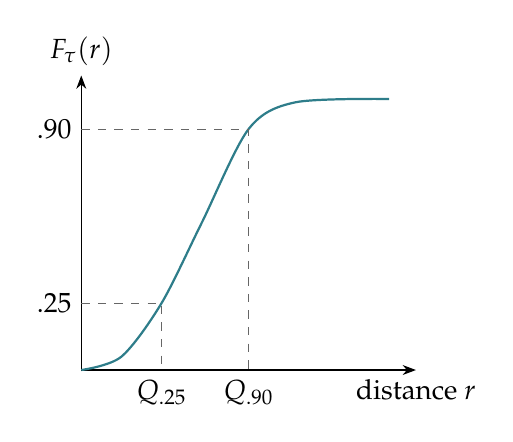
\begin{tikzpicture}[x=.85cm,y=.85cm,>=Stealth]
 \draw[->](0,0)--(5,0)node[below]{distance $r$};
 \draw[->](0,0)--(0,4.4)node[above]{$F_\tau(r)$};
 \draw[teal,thick]plot[smooth]coordinates{(0,0)(.6,.2)(1.2,1)(1.8,2.2)(2.5,3.6)(3.2,4)(4.6,4.05)};
 \draw[muted,dashed](0,1)--(1.2,1)--(1.2,0);
 \draw[muted,dashed](0,3.6)--(2.5,3.6)--(2.5,0);
 \node[left]at(0,1){$.25$};\node[left]at(0,3.6){$.90$};
 \node[below]at(1.2,0){$Q_{.25}$};\node[below]at(2.5,0){$Q_{.90}$};
\end{tikzpicture}
\end{columns}
\source{Schematic CDF. Quantiles describe ranks within one distribution; they do not define permanent classes of slow and fast flights. Equal slopes are necessary, not sufficient, for process self-similarity.}
\timing{1:00}{The lower quartile probes relatively small displacements, while the 90th percentile probes larger ones. Both use the same distribution at each lag. A different flight may supply an observation near each rank, and rank identities may change; that does not invalidate a quantile. The mathematical issue is whether the population and weighting used to construct the distribution change with lag. No isotropy assumption is needed for the radial scaling implication.}
\end{frame}

\begin{frame}{Controlling the population changes the quantile result}
\centering\fig[47mm]{talk-quantile-slopes.pdf}
\small\raggedright
\textbf{Fixed control:} the same flights, equal flight weights and the same origins at every lag.
The long cohorts contain \kw{107 para / 56 hang flights} with segments $\ge20,000$ s.
\source{The changing para pool gives $H_{.90}>H_{.25}$; the fixed control gives the reverse. Intermediate weight/origin controls are in the \hyperlink{quantile-backup}{backup figure}. Slopes are descriptive.}
\timing{1:20}{This is a resolved methodological concern with an unresolved inferential consequence. The fully controlled empirical CDF averages within each fixed flight and then gives each flight equal weight. The same admissible origins, whose longest-lag increment remains in the segment, are used at every lag. The four controls separate cohort membership, weights and origins. In the fixed para cohort the lower and upper slopes are 0.979 and 0.892; in hang they are 0.995 and 0.864. They are not strictly monotone across all ranks. These unusually long flights need not represent shorter flights. Overlapping origins do not provide independent replications.}
\end{frame}

\begin{frame}{Relative spread changes, but the change is not monotone}
\begin{columns}[c,onlytextwidth]
\column{.65\textwidth}\fig[48mm]{talk-quantile-ratio.pdf}
\column{.32\textwidth}
\small
\[
 \begin{aligned}
 &\frac{d\log(Q_{.90}/Q_{.25})}{d\log\tau}\\
 &\qquad=H_{.90}(\tau)-H_{.25}(\tau).
 \end{aligned}
\]
The ratio first rises, then falls, then rises again.\par\medskip
A negative fitted slope summarizes part of that evolution; it does not imply narrowing at every lag.
\end{columns}
\question{How much of this shape evolution survives site--day uncertainty, route matching and phase conditioning?}
\source{Fully controlled population. A lower ratio means less relative spread by this measure; it does not establish a flatter density tail.}
\timing{1:00}{At 10 seconds the ratios are about 1.94 and 2.23; they peak around 80 seconds at 4.48 and 5.89, fall towards 2000 seconds, and rise again. At 10000 seconds they are about 3.03 and 2.65, above the initial values. Because OLS is linear in the logarithmic observations, the fitted log-ratio slope equals the difference of fitted quantile slopes on the same lag set. This identity does not imply monotonicity. Both quantiles can grow while their ratio falls.}
\end{frame}

\begin{frame}{The Pyrenean archive has a strong east--west preference}
\begin{columns}[c,onlytextwidth]
\column{.65\textwidth}
\fig[26mm]{terrain-position.pdf}\par\vspace{1mm}
\fig[26mm]{terrain-velocity.pdf}
\column{.32\textwidth}
\small
\[
 A_u(t)=\frac{\langle u_E(t)^2\rangle}{\langle u_N(t)^2\rangle}.
\]
\textbf{Elapsed time since launch}, not displacement lag.\par\medskip
Position ratio approaches five in the Pyrenees. Velocity is also directionally unbalanced.\par\medskip
These uncentred moments include mean motion.
\end{columns}
\source{Paraglider archive; take-off regions. Pointwise 10--90\% site--day bootstrap bands; at least 30 flights / 10 groups at each time. Directional balance is weaker than full isotropy.}
\timing{1:00}{Keep the clock distinction explicit: these kinematics figures use elapsed time since launch, while the preceding increment statistics use lag. The Pyrenean position ratio grows towards five. That is consistent with the east--west development of the massif, but routes, launch-site selection, weather and disappearing short flights can all contribute. The regional bootstrap bands already exist; they do not provide confidence intervals for the quantile slopes shown earlier. A ratio of one would not test cross-covariance or the entire angular distribution.}
\end{frame}

\begin{frame}{The experience contrast depends on region and elapsed time}
\begin{columns}[c,onlytextwidth]
\column{.49\textwidth}\centering\fig[49mm]{equipment-alps.pdf}
\column{.49\textwidth}\centering\fig[49mm]{equipment-pyrenees.pdf}
\end{columns}
\small
In the Alps the expert proxy is more balanced. In the Pyrenees the curves cross; there is no uniform expert advantage.
\source{Beginners = EN A/B (violet); experts = EN C/D/CCC (ochre). Equipment is an experience proxy, not an individual skill measurement. Same ratio and clock as the previous slide.}
\timing{1:00}{Use the user's proposed class mapping, with its limitation stated plainly. An experienced pilot may fly an A/B wing, and equipment performance itself changes the dynamics. In the Alps the expert group has a position ratio closer to one. In the Pyrenees the ordering changes after a few hundred seconds and both groups reach large east--west ratios. We should therefore show the regional result rather than claim that experts generally overcome terrain constraints. A matched site--day analysis is the next useful contrast.}
\end{frame}

\begin{frame}{PCA describes preferred axes; wind needs independent information}
\begin{columns}[T,onlytextwidth]
\column{.47\textwidth}
\textbf{A rotation preserves distance}\par
\[
 \Sigma=U\Lambda U^\top,\qquad |U^\top\mathbf X|=|\mathbf X|.
\]
\small PCA decorrelates components at a chosen lag. It cannot repair radial collapse or remove temporal dependence.\par\medskip
Whitening changes lengths and only fixes second moments at the fitted scale.
\column{.49\textwidth}
\textbf{Ground velocity has two unknown terms}\par
\[
 \mathbf v_{\rm ground}=\mathbf v_{\rm air}+\mathbf w_h.
\]
\small Terrain constrains headings; wind also changes position. Differentiation does not separate the two.\par\medskip
Different marginal exponents, or changing joint dependence, can prevent radial scaling.
\end{columns}
\question{Choose matched environments and an independent wind estimate before defining an ``environment-free'' model target.}
\source{\hyperlink{pca-backup}{Regional PCA and its numerical support}. Anisotropy alone is compatible with a self-similar vector and a self-similar radius.}
\timing{1:00}{Even independent Gaussian components can yield a changing radial exponent if their component exponents differ. If both component exponents agree, changing dependence can still prevent joint scaling. Conversely, a joint vector scaling law always implies radial scaling, whether the vector is isotropic or not. Rotating each flight randomly would balance aggregate directions without changing radial displacements; it cannot recover still-air motion. Independent wind information or carefully justified phase-based wind estimates should be discussed before choosing an environmental correction.}
\end{frame}

\begin{frame}{The moment spectrum challenges a specific L\'evy-walk benchmark}
\begin{columns}[c,onlytextwidth]
\column{.55\textwidth}\fig[49mm]{talk-moments.pdf}
\column{.42\textwidth}
\small
$M_q=\langle R^q\rangle\propto\tau^{\zeta(q)}$.\par\medskip
For a constant-speed renewal walk with isotropic independent headings and $\psi(t)\sim t^{-1-\beta}$, $1<\beta<2$:
\[
 \zeta_{\rm LW}(q)=
 \begin{cases}q/\beta,&q<\beta,\\q+1-\beta,&q>\beta.\end{cases}
\]
The empirical spectrum is nearly linear over $q=0.25$--4.
\end{columns}
\question{Can finite-record simulations resolve the predicted branch change under our sampling and selection?}
\source{Pooled windows. $\beta=1.5$ is illustrative, not a fitted null; $q=\beta$ has a logarithmic correction. \href{https://doi.org/10.1103/RevModPhys.87.483}{Zaburdaev, Denisov \& Klafter (2015)}.}
\timing{1:20}{The reported zeta(2) values are 1.733 and 1.693, different from equal-flight V1 because the weights differ. Nu(q)=zeta(q)/q varies only modestly: 0.849--0.878 for para and 0.839--0.861 for hang. This looks unlike the two-branch asymptotic benchmark, but it is not a calibrated exclusion. The reference beta is not estimated from our data. Fit candidate parameters, simulate comparable lengths and cadence, and compare moments together with controlled quantiles. High-order moments need checks for domination by a few flights. Truncation and correlated legs are different candidate models.}
\end{frame}

\begin{frame}{Velocity memory persists after averaging over minutes}
\begin{columns}[c,onlytextwidth]
\column{.61\textwidth}\fig[47mm]{memory-positive.pdf}
\column{.36\textwidth}
\small
\[
 \mathbf v_h(t)=\frac{\mathbf r(t+h)-\mathbf r(t)}{h}.
\]
For $h=10,60,300$ s.\par\medskip
Mean of per-flight centred, normalized correlations.\par\medskip
At 600 s, para correlations are $0.144$, $0.198$, $0.272$ for the three widths.
\end{columns}
\question{A finite-persistence model remains plausible: fit its MSD and coarse velocity correlations jointly.}
\source{Teal: 10 s; plum dashed: 60 s; grey dotted: 300 s. Positive values shown; \hyperlink{memory-backup}{signed curves in backup}. Curvature prevents a single decay-law claim.}
\timing{1:20}{Velocities come from adjacent non-overlapping blocks; separations are at least h and at most a quarter of each contributing record. At least 20 flights contribute. The plotted quantity is the equal-flight mean of normalized correlations, not a pooled covariance. Finite-record centring can depress long-lag values, and the hang curve becomes negative. An exponential stationary covariance produces an MSD that crosses from ballistic to diffusive, so a fitted exponent between one and two is compatible with finite persistence. Averaging suppresses fast fluctuations and can raise the normalized correlation without lengthening the underlying memory time.}
\end{frame}

\begin{frame}{Non-Gaussian pooled increments can arise from Gaussian mixtures}
\begin{columns}[c,onlytextwidth]
\column{.56\textwidth}\fig[48mm]{talk-kurtosis.pdf}
\column{.41\textwidth}
\small
\[
 \begin{aligned}
 \mathbf Z&=\Sigma^{-1/2}(\mathbf X-\bm\mu),\\
 K_M&=\langle|\mathbf Z|^4\rangle-8.
 \end{aligned}
\]
A nonsingular 2D Gaussian has $K_M=0$, including anisotropic Gaussians.\par\medskip
The observed curve changes sign and rises at large lag, where support is weakest.
\end{columns}
\question{Test Gaussianity within matched environments or phases before rejecting conditional Gaussian dynamics.}
\source{Centred, full-covariance Mardia excess; pooled windows. Positive excess does not identify a power-law tail. \href{https://doi.org/10.1093/biomet/57.3.519}{Mardia (1970)}.}
\timing{0:50}{Explain the full covariance normalization: unequal east and north variances alone do not produce a nonzero population excess for a Gaussian. But mixing Gaussian variances does. If X equals sqrt(A) times a fixed Gaussian vector, K equals eight times Var(A) divided by E(A) squared. This illustrates heterogeneity; it is not a correction formula for arbitrary flights. The finite-sample estimate need not vanish even for Gaussian data, and overlapping windows require a matched reference before significance claims.}
\end{frame}

\begin{frame}{Long flights occur in both equipment groups}
\centering\fig[45mm]{talk-duration.pdf}
\small\raggedright
For $T\ge4$ h: \textcolor{beginner}{7,426 beginners} and \textcolor{expert}{27,842 experts}.\par
Across 10--10,000 s, all-duration slopes are \textcolor{beginner}{\StatDurationABFullExponent}\ and \textcolor{expert}{\StatDurationCDCCCFullExponent}.
\source{Equal-flight MSD; groups are nested. Threshold curves stop at $\tau=T_0/2$; at least 30 flights per lag. \hyperlink{duration-backup}{All counts and common-range slopes}.}
\timing{1:10}{The hypothesis that only experts contribute to flights longer than four hours is contradicted by the counts. Experts nevertheless become more frequent in the long-duration groups. On the common 10--1695 second interval, expert slopes exceed beginner slopes in every duration cell; within both classes slopes also increase between all flights and the four-hour group. This shorter interval is needed to compare all four nested cohorts under the half-duration rule. It is distinct from the main three-decade fit. Equipment, pilot selection, region and weather remain possible causes.}
\end{frame}

\begin{frame}{Fixing equipment proportions removes part of the duration contrast}
\begin{columns}[c,onlytextwidth]
\column{.57\textwidth}\fig[47mm]{talk-composition.pdf}
\column{.40\textwidth}
\small
\[
 M_{T_0}^{\rm fixed}(\tau)=\sum_c\pi_c M_{T_0,c}(\tau).
\]
Fixed weights: $\pi_{\rm A/B}=0.365$, $\pi_{\rm C/D/CCC}=0.635$.\par\medskip
At $\tau=1695$ s the ratio falls from $1.42$ to $1.35$. A within-class contrast remains.
\end{columns}
\question{Match site--day and task next. Convergence near 7200 s also reflects shorter flights leaving the reference.}
\source{Both curves use the same two known equipment groups. Equality at one lag does not establish independence from flight duration.}
\timing{0:50}{The expert fraction among known classes rises from 63.5 percent overall to 78.9 percent in the four-hour cohort. Standardization uses the all-duration proportions at every lag for both numerator and denominator. It is a descriptive reweighting, not a causal adjustment. The remaining difference shows that the two-class proportions alone cannot account for the observed amplitude contrast. Near half the duration threshold, the reference loses shorter flights, so the curves are increasingly comparing similar populations.}
\end{frame}

\begin{frame}{Which models are challenged, and which remain open?}
\small\renewcommand{\arraystretch}{1.2}\setlength{\tabcolsep}{4pt}
\begin{tabular}{@{}>{\raggedright\arraybackslash}p{.26\textwidth}>{\raggedright\arraybackslash}p{.34\textwidth}>{\raggedright\arraybackslash}p{.35\textwidth}@{}}\toprule
Candidate & Prediction to test & Present conclusion\\\midrule
Homogeneous Brownian & Linear MSD; independent increments & Challenged over the measured range.\\
Constant drift + Brownian & Drift-free $V_2\propto\tau$ & Simple version challenged; mixtures unresolved.\\
Homogeneous fBm & Gaussian law; common $H_p$ & Challenged as one pooled law.\\
Exponential velocity memory & Ballistic--diffusive crossover & Remains a candidate.\\
Renewal L\'evy walk, $1<\beta<2$ & Two-branch moment spectrum & Finite-record comparison still needed.\\\bottomrule
\end{tabular}
\question{``Challenged'' means a descriptive mismatch. Calibrated statistical rejection is still to be done.}
\source{Each candidate needs its own parameters, environmental assumptions and observation protocol. A long-time diffusive limit has not been tested.}
\timing{1:00}{This table is deliberately more cautious than the older slides. Ordinary Brownian motion is a poor descriptive model of the observed interval, but the asymptotic regime is unknown. fBm is challenged as a homogeneous pooled law; a phase-conditioned or environmentally heterogeneous Gaussian construction is not excluded. The exponential-persistence candidate deserves a joint MSD and VACF comparison. Standard Lévy walk needs finite-record calibration rather than rejection from an illustrative asymptotic line. An unbounded Lévy flight cannot literally describe continuous finite-speed flight; effective truncated versions need separate predictions.}
\end{frame}

\begin{frame}{Three decisions for this meeting}
\begin{enumerate}
 \item \kw{Define the model target.}\par
 \small Ground-relative motion conditional on environment, or a residual after an independently justified wind correction?
 \normalsize
 \item \kw{Agree the first calibrated comparisons.}\par
 \small Fit Brownian controls, fBm, finite persistence and a specified L\'evy walk; simulate the same record lengths, selection and estimators.
 \normalsize
 \item \kw{Choose the most informative next measurements.}\par
 \small Site--day uncertainty and route matching now; phase durations, increments and between-phase dependence after segmentation validation.
\end{enumerate}
\question{We have measured constraints on growth, shape, geometry and memory. The generating process and an intrinsic Hurst exponent remain unresolved.}
\timing{2:20}{Use the remaining time to ask for prioritization. First agree what the stochastic model should represent; no isotropization operation has yet recovered still-air motion. Second agree a small set of explicit null models and jointly assessed observables rather than a search for as many nominal rejections as possible. Third agree the observational unit for uncertainty and the phase-conditioned measurements that distinguish renewal from correlated episodes. The future physical model chapter will also compare Monte Carlo simulations to global and phase-conditioned data, but null calibration for this chapter can begin earlier. Stop the prepared talk here and use backup slides only in response to questions.}
\end{frame}

\backupstart
\begin{frame}[label=quantile-backup]{The four population controls}
\begin{columns}[c,onlytextwidth]
\column{.56\textwidth}\fig[62mm]{ch3_quantile_control.pdf}
\column{.41\textwidth}\small
\begin{enumerate}
\item All available flights, pooled windows.
\item Fixed long flights, pooled windows.
\item Fixed flights, equal flight weights.
\item Same flights, weights and origins.
\end{enumerate}
\[
 \widehat F_\tau(x)=\frac1{N_*}\sum_f\frac1{n_f^*}
 \sum_k\mathbf1\{R_{fk}(\tau)\le x\}.
\]
Overlapping origins remain dependent.
\end{columns}
\end{frame}

\begin{frame}{An example of changing shape at fixed quantile ranks}
\begin{columns}[c,onlytextwidth]
\column{.56\textwidth}\fig[61mm]{quantile_scaling_schematic.pdf}
\column{.41\textwidth}\small
\[
 R(\tau)=(\tau/\tau_0)^{.85}e^{\sigma(\tau)Z},\quad Z\sim N(0,1),
\]
\[
 \sigma(\tau)=.9-.1\log(\tau/\tau_0),
\]
\[
 H_p=.85-.1\Phi^{-1}(p).
\]
All shown quantiles grow, while spread relative to the median shrinks.\par\medskip
Analytical illustration only; this is not a fitted model for flights.
\end{columns}
\end{frame}

\begin{frame}[label=circle]{A circle retains its geometry after second differencing}
\begin{columns}[c,onlytextwidth]
\column{.54\textwidth}\fig[59mm]{closed_loop_schematic.pdf}
\column{.43\textwidth}\small
\[
 \mathbf r(t)=a(\cos\omega t,\sin\omega t),\quad T_c=2\pi/\omega,
\]
\[
 V_1=4a^2\sin^2(\pi\tau/T_c),
\]
\[
 V_2=16a^2\sin^4(\pi\tau/T_c).
\]
The periodic continuation defines $V_2$ across the illustrated lags. Constant speed does not imply ballistic displacement at every lag.
\end{columns}
\source{Exact geometrical example, not an empirical estimate.}
\end{frame}

\begin{frame}[label=memory-backup]{Signed memory and the finite-persistence alternative}
\begin{columns}[c,onlytextwidth]
\column{.55\textwidth}\fig[49mm]{memory-signed.pdf}
\column{.42\textwidth}\small
For the same stationary, centred velocity population,
\[
 M_{2,c}(\tau)=2\sigma_v^2\int_0^\tau(\tau-s)C(s)\,ds.
\]
With $C(s)=e^{-s/t_p}$,
\[
 M_{2,c}=2\sigma_v^2t_p[\tau-t_p(1-e^{-\tau/t_p})].
\]
Ballistic at short times, diffusive at long times.
\end{columns}
\source{\href{https://doi.org/10.1112/plms/s2-20.1.196}{Taylor (1922)}, pp. 207--208. This covariance identity cannot be applied directly to differently weighted heterogeneous means.}
\end{frame}

\begin{frame}[label=pca-backup]{Regional principal axes are lag-dependent descriptive measurements}
\centering\fig[47mm]{talk-pca.pdf}
\small\raggedright
Paragliders at $\tau=1070$ s. Covariance ellipses are normalized by their trace to compare shape and direction, without changing their eigenvalue ratios.
\source{Centred covariance of pooled windows; dashed line = principal axis modulo $180^\circ$. Ellipses describe second moments, not Gaussian confidence regions. The coast is a small subgroup and is not an established isotropic control.}
\end{frame}

\begin{frame}[label=duration-backup]{Duration and equipment on the common 10--1695 s interval}
\centering\small\renewcommand{\arraystretch}{1.12}
% Generated by scripts/reporting/ch3_global_transport/generate_duration_equipment.py
\begin{tabular}{@{}llrrr@{}}
\toprule
Experience proxy & Duration & Flights & $b$ & RMS residual (dex) \\
\midrule
Beginners & All & 54,292 & 1.755 & 0.022 \\
Beginners & $T\ge1$ h & 51,124 & 1.754 & 0.022 \\
Beginners & $T\ge2$ h & 31,768 & 1.767 & 0.020 \\
Beginners & $T\ge4$ h & 7,415 & 1.806 & 0.017 \\
\addlinespace
Experts & All & 94,283 & 1.803 & 0.017 \\
Experts & $T\ge1$ h & 91,182 & 1.802 & 0.017 \\
Experts & $T\ge2$ h & 69,087 & 1.811 & 0.016 \\
Experts & $T\ge4$ h & 27,815 & 1.836 & 0.015 \\
\addlinespace
\bottomrule
\end{tabular}

\source{Counts are eligible flights, not independent windows; support falls with lag. RMS residual measures departures from a fitted line, not uncertainty. Threshold samples overlap.}
\end{frame}

\begin{frame}{Sources and the scope of the evidence}
\small
\refitem{https://doi.org/10.1103/RevModPhys.87.483}{Zaburdaev, Denisov \& Klafter (2015), \emph{L\'evy walks}}{Moment-spectrum benchmark}
\refitem{https://doi.org/10.1137/1010093}{Mandelbrot \& Van Ness (1968), \emph{Fractional Brownian motions}}{fBm construction}
\refitem{https://doi.org/10.1112/plms/s2-20.1.196}{Taylor (1922), \emph{Diffusion by continuous movements}}{Velocity/displacement relation}
\refitem{https://doi.org/10.1093/biomet/57.3.519}{Mardia (1970), \emph{Measures of multivariate skewness and kurtosis}}{Centred kurtosis}
\refitem{https://doi.org/10.1214/aos/1176344552}{Efron (1979), \emph{Bootstrap methods}}{Resampling principle}
\source{Numerical evidence: current Chapter 3 reports, frozen in the accompanying data and asset manifests. Bibliographic access limitations are retained in the repository audit; citations do not validate the chosen sampling design or constitute calibrated rejection tests.}
\end{frame}
\end{document}
